\documentclass{standalone}
\usepackage{tikz}
\usetikzlibrary{patterns, positioning}

\begin{document}
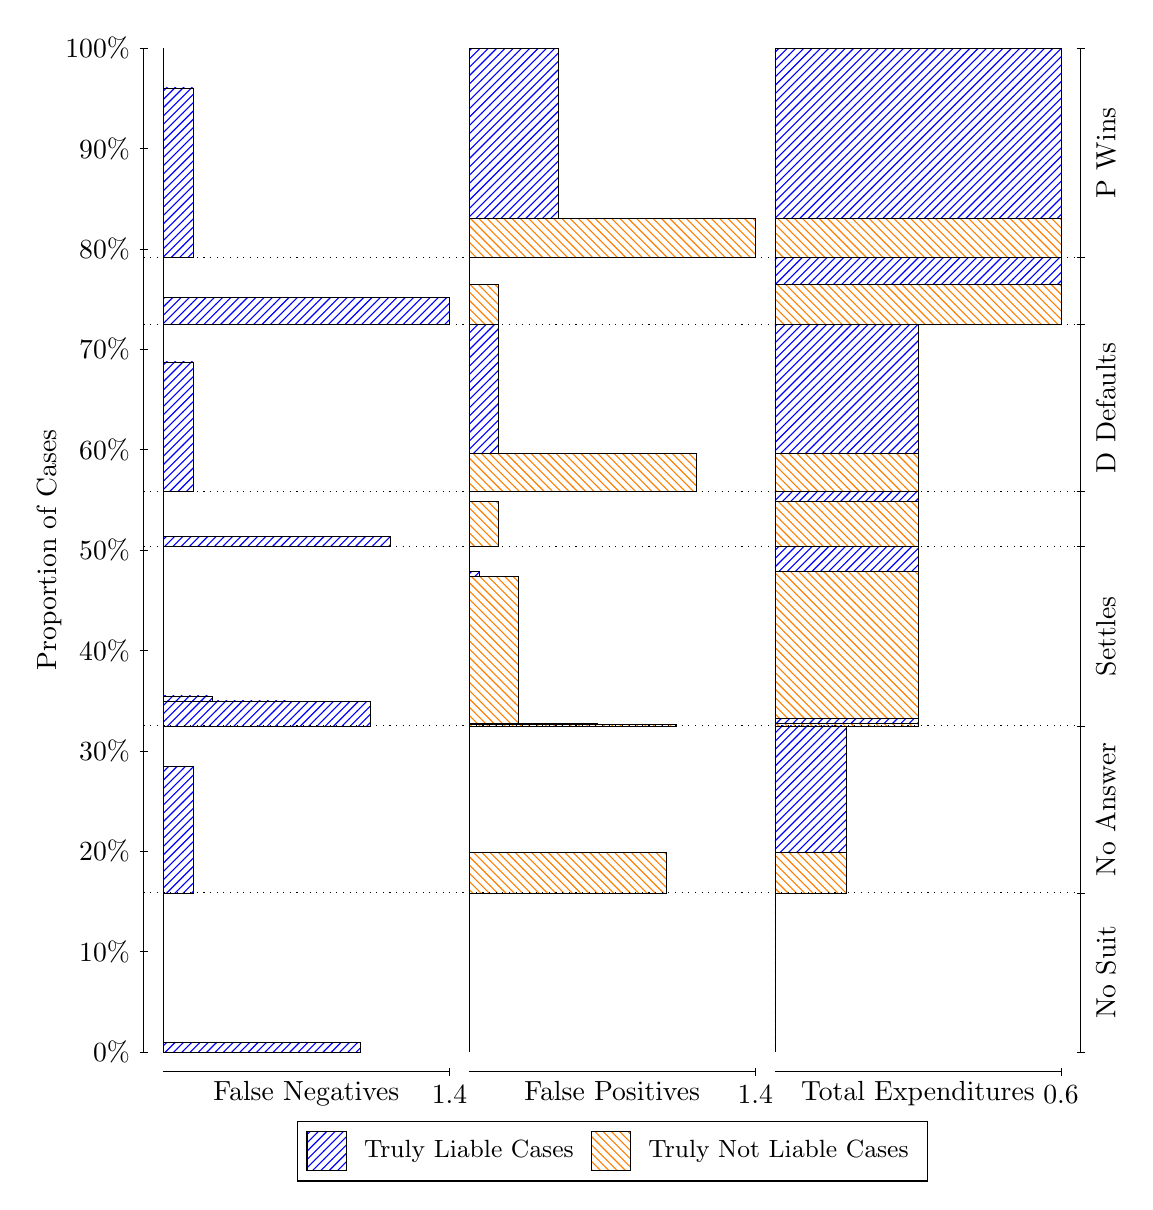
\begin{tikzpicture}
\draw[black, very thin] (1.5,1.75) -- (1.5,14.5);
\node[rotate=90, anchor=center] at (0.3, 8.125) {Proportion of Cases};
\draw[black, very thin] (1.45,1.75) -- (1.55,1.75);
\node[anchor=east] at (1.45, 1.75) {0\%};
\draw[black, very thin] (1.45,3.025) -- (1.55,3.025);
\node[anchor=east] at (1.45, 3.025) {10\%};
\draw[black, very thin] (1.45,4.3) -- (1.55,4.3);
\node[anchor=east] at (1.45, 4.3) {20\%};
\draw[black, very thin] (1.45,5.575) -- (1.55,5.575);
\node[anchor=east] at (1.45, 5.575) {30\%};
\draw[black, very thin] (1.45,6.85) -- (1.55,6.85);
\node[anchor=east] at (1.45, 6.85) {40\%};
\draw[black, very thin] (1.45,8.125) -- (1.55,8.125);
\node[anchor=east] at (1.45, 8.125) {50\%};
\draw[black, very thin] (1.45,9.4) -- (1.55,9.4);
\node[anchor=east] at (1.45, 9.4) {60\%};
\draw[black, very thin] (1.45,10.675) -- (1.55,10.675);
\node[anchor=east] at (1.45, 10.675) {70\%};
\draw[black, very thin] (1.45,11.95) -- (1.55,11.95);
\node[anchor=east] at (1.45, 11.95) {80\%};
\draw[black, very thin] (1.45,13.225) -- (1.55,13.225);
\node[anchor=east] at (1.45, 13.225) {90\%};
\draw[black, very thin] (1.45,14.5) -- (1.55,14.5);
\node[anchor=east] at (1.45, 14.5) {100\%};

\draw[black, very thin] (13.4,1.75) -- (13.4,14.5);
\draw[black, very thin] (13.35,1.75) -- (13.45,1.75);
\node[anchor=west] at (13.35, 1.75) {};
\draw[black, very thin] (13.35,3.7703) -- (13.45,3.7703);
\node[anchor=west] at (13.35, 3.7703) {};
\draw[black, very thin] (13.35,5.8914) -- (13.45,5.8914);
\node[anchor=west] at (13.35, 5.8914) {};
\draw[black, very thin] (13.35,8.1676) -- (13.45,8.1676);
\node[anchor=west] at (13.35, 8.1676) {};
\draw[black, very thin] (13.35,8.8698) -- (13.45,8.8698);
\node[anchor=west] at (13.35, 8.8698) {};
\draw[black, very thin] (13.35,10.993) -- (13.45,10.993);
\node[anchor=west] at (13.35, 10.993) {};
\draw[black, very thin] (13.35,11.837) -- (13.45,11.837);
\node[anchor=west] at (13.35, 11.837) {};
\draw[black, very thin] (13.35,14.5) -- (13.45,14.5);
\node[anchor=west] at (13.35, 14.5) {};

\draw[black, very thin, pattern color=blue, pattern=north east lines] (1.75,1.75) rectangle (4.2557,1.8684);
\draw[black, very thin, pattern color=orange, pattern=north west lines] (1.75,1.8684) rectangle (1.75,3.7703);
\draw[black, very thin, pattern color=blue, pattern=north east lines] (1.75,3.7703) rectangle (2.1259,5.3798);
\draw[black, very thin, pattern color=orange, pattern=north west lines] (1.75,5.3798) rectangle (1.75,5.8914);
\draw[black, very thin, pattern color=blue, pattern=north east lines] (1.75,5.8914) rectangle (4.381,6.2054);
\draw[black, very thin, pattern color=blue, pattern=north east lines] (1.75,6.2054) rectangle (3.3787,6.2078);
\draw[black, very thin, pattern color=blue, pattern=north east lines] (1.75,6.2078) rectangle (2.3764,6.2714);
\draw[black, very thin, pattern color=orange, pattern=north west lines] (1.75,6.2714) rectangle (1.75,8.1676);
\draw[black, very thin, pattern color=blue, pattern=north east lines] (1.75,8.1676) rectangle (4.6316,8.2932);
\draw[black, very thin, pattern color=orange, pattern=north west lines] (1.75,8.2932) rectangle (1.75,8.8698);
\draw[black, very thin, pattern color=blue, pattern=north east lines] (1.75,8.8698) rectangle (2.1259,10.514);
\draw[black, very thin, pattern color=orange, pattern=north west lines] (1.75,10.514) rectangle (1.75,10.993);
\draw[black, very thin, pattern color=blue, pattern=north east lines] (1.75,10.993) rectangle (5.3833,11.332);
\draw[black, very thin, pattern color=orange, pattern=north west lines] (1.75,11.332) rectangle (1.75,11.837);
\draw[black, very thin, pattern color=blue, pattern=north east lines] (1.75,11.837) rectangle (2.1259,13.995);
\draw[black, very thin, pattern color=orange, pattern=north west lines] (1.75,13.995) rectangle (1.75,14.5);
\draw[black, very thin, pattern color=orange, pattern=north west lines] (5.6333,1.75) rectangle (5.6333,3.6518);
\draw[black, very thin, pattern color=blue, pattern=north east lines] (5.6333,3.6518) rectangle (5.6333,3.7703);
\draw[black, very thin, pattern color=orange, pattern=north west lines] (5.6333,3.7703) rectangle (8.1391,4.2819);
\draw[black, very thin, pattern color=blue, pattern=north east lines] (5.6333,4.2819) rectangle (5.6333,5.8914);
\draw[black, very thin, pattern color=orange, pattern=north west lines] (5.6333,5.8914) rectangle (8.2644,5.9114);
\draw[black, very thin, pattern color=orange, pattern=north west lines] (5.6333,5.9114) rectangle (7.2621,5.9229);
\draw[black, very thin, pattern color=orange, pattern=north west lines] (5.6333,5.9229) rectangle (6.2598,7.7876);
\draw[black, very thin, pattern color=blue, pattern=north east lines] (5.6333,7.7876) rectangle (5.7586,7.8512);
\draw[black, very thin, pattern color=blue, pattern=north east lines] (5.6333,7.8512) rectangle (5.6333,8.1676);
\draw[black, very thin, pattern color=orange, pattern=north west lines] (5.6333,8.1676) rectangle (6.0092,8.7442);
\draw[black, very thin, pattern color=blue, pattern=north east lines] (5.6333,8.7442) rectangle (5.6333,8.8698);
\draw[black, very thin, pattern color=orange, pattern=north west lines] (5.6333,8.8698) rectangle (8.5149,9.3487);
\draw[black, very thin, pattern color=blue, pattern=north east lines] (5.6333,9.3487) rectangle (6.0092,10.993);
\draw[black, very thin, pattern color=orange, pattern=north west lines] (5.6333,10.993) rectangle (6.0092,11.498);
\draw[black, very thin, pattern color=blue, pattern=north east lines] (5.6333,11.498) rectangle (5.6333,11.837);
\draw[black, very thin, pattern color=orange, pattern=north west lines] (5.6333,11.837) rectangle (9.2667,12.341);
\draw[black, very thin, pattern color=blue, pattern=north east lines] (5.6333,12.341) rectangle (6.7609,14.5);
\draw[black, very thin, pattern color=orange, pattern=north west lines] (9.5167,1.75) rectangle (9.5167,3.6518);
\draw[black, very thin, pattern color=blue, pattern=north east lines] (9.5167,3.6518) rectangle (9.5167,3.7703);
\draw[black, very thin, pattern color=orange, pattern=north west lines] (9.5167,3.7703) rectangle (10.425,4.2819);
\draw[black, very thin, pattern color=blue, pattern=north east lines] (9.5167,4.2819) rectangle (10.425,5.8914);
\draw[black, very thin, pattern color=orange, pattern=north west lines] (9.5167,5.8914) rectangle (11.333,5.9229);
\draw[black, very thin, pattern color=blue, pattern=north east lines] (9.5167,5.9229) rectangle (11.333,5.989);
\draw[black, very thin, pattern color=orange, pattern=north west lines] (9.5167,5.989) rectangle (11.333,7.8536);
\draw[black, very thin, pattern color=blue, pattern=north east lines] (9.5167,7.8536) rectangle (11.333,8.1676);
\draw[black, very thin, pattern color=orange, pattern=north west lines] (9.5167,8.1676) rectangle (11.333,8.7442);
\draw[black, very thin, pattern color=blue, pattern=north east lines] (9.5167,8.7442) rectangle (11.333,8.8698);
\draw[black, very thin, pattern color=orange, pattern=north west lines] (9.5167,8.8698) rectangle (11.333,9.3487);
\draw[black, very thin, pattern color=blue, pattern=north east lines] (9.5167,9.3487) rectangle (11.333,10.993);
\draw[black, very thin, pattern color=orange, pattern=north west lines] (9.5167,10.993) rectangle (13.15,11.498);
\draw[black, very thin, pattern color=blue, pattern=north east lines] (9.5167,11.498) rectangle (13.15,11.837);
\draw[black, very thin, pattern color=orange, pattern=north west lines] (9.5167,11.837) rectangle (13.15,12.341);
\draw[black, very thin, pattern color=blue, pattern=north east lines] (9.5167,12.341) rectangle (13.15,14.5);
\draw[black, dotted] (1.5,3.7703) -- (13.4,3.7703);
\draw[black, dotted] (1.5,5.8914) -- (13.4,5.8914);
\draw[black, dotted] (1.5,8.1676) -- (13.4,8.1676);
\draw[black, dotted] (1.5,8.8698) -- (13.4,8.8698);
\draw[black, dotted] (1.5,10.993) -- (13.4,10.993);
\draw[black, dotted] (1.5,11.837) -- (13.4,11.837);
\draw[black, very thin] (1.75,1.5) -- (5.3833,1.5);
\node[anchor=north] at (3.5667, 1.5) {False Negatives};
\draw[black, very thin] (5.3833,1.45) -- (5.3833,1.55);
\node[anchor=north] at (5.3833, 1.45) {1.4};

\draw[black, very thin] (5.6333,1.5) -- (9.2667,1.5);
\node[anchor=north] at (7.45, 1.5) {False Positives};
\draw[black, very thin] (9.2667,1.45) -- (9.2667,1.55);
\node[anchor=north] at (9.2667, 1.45) {1.4};

\draw[black, very thin] (9.5167,1.5) -- (13.15,1.5);
\node[anchor=north] at (11.333, 1.5) {Total Expenditures};
\draw[black, very thin] (13.15,1.45) -- (13.15,1.55);
\node[anchor=north] at (13.15, 1.45) {0.6};

\node[black, centered, rotate=90] at (13.72, 2.7601) {No Suit};
\node[black, centered, rotate=90] at (13.72, 4.8308) {No Answer};
\node[black, centered, rotate=90] at (13.72, 7.0295) {Settles};

\node[black, centered, rotate=90] at (13.72, 9.9315) {D Defaults};

\node[black, centered, rotate=90] at (13.72, 13.168) {P Wins};

\draw (7.449999999999999,1.5) node[draw=none] (baseCoordinate) {};
\begin{scope}[align=center]
        \matrix[scale=0.5, draw=black, below=0.5cm of baseCoordinate, nodes={draw}, column sep=0.1cm]{
            \node[rectangle, draw, minimum width=0.5cm, minimum height=0.5cm, pattern=north east lines, pattern color=blue] {}; &
            \node[draw=none, font=\small] (B) {Truly Liable Cases}; &
            \node[rectangle, draw, minimum width=0.5cm, minimum height=0.5cm, pattern=north west lines, pattern color=orange] {}; &
            \node[draw=none, font=\small] (B) {Truly Not Liable Cases}; \\
            };
\end{scope}

\end{tikzpicture}
\end{document}